\chapter{Targeting the Non-Excluded pMSSM with Multivariate Discriminants}
\label{chap:money}

Designing analyses to target the non-excluded regions of the pMSSM is challenging for a number of reasons. The fact that the signal events in this subset contain soft objects and low $\met$ means that the observables typically used to distinguish between \SM~backgrounds and the signal no longer function as excellent discriminators. 

However, the situation is not completely dire. The  $\Ht$, $\met$, and the prevalence of high $p_{T}$ objects are popular largely because they exploit well-understood differences between typical new physics signals and background. There are presumably other event characteristics that differ between events arising from supersymmetry and those from standard model processes, such as the relative angles between particles, the presence and characteristics of leptons and heavy-flavor quarks in the events, as well as various combinations of the four-vector components of particles. Information not considered in most searches, but to which we have ready access, include the $\pt$, $\eta$, and $\phi$ of particles in the event. Correlations among these observables may serve to distinguish between standard model events and BSM events.

In the next section, the methods detailed in this document are combined into an outline for a set of possible strategies for targeting non-excluded SUSY models that predict large cross sections in the most challenging all-hadronic kinematic regions: those of low $\met$, where QCD is the dominant background, and low $\Ht$, where $\zinv$ events are the dominant background. Multivariate methods are used to build discriminants that increase the sensitivity to supersymmetry models in these regions. Then, Section \ref{sec:lastbattle} presents a preliminary analysis that has been carried out following one such strategy. 

\section{Methods for exploring difficult pMSSM points}

Can our sensitivity to the pMSSM be increased through the use of multivariate discriminants? in order to proceed, answering the following questions is key:
\begin{enumerate}
\item Does the set of particle four-vectors in an event contain additional information that distinguishes signal from background events?
\item Can this information be accurately modeled in real and simulated events?
\item Is any such discrimination power generalizable to a large class of interesting models, or is it limited to a narrowly-defined subset of models or even a single model?
\end{enumerate}
I set out to answer these questions by considering events in two background-dominated kinematic signal regions, corresponding to modified versions of the baseline selection of the CMS multi-jet $+$ $\mht$ search \cite{Khachatryan:2016kdk}. The fist signal region is taken to be the low-$\mht$ sideband of the baseline selection \cite{Khachatryan:2016kdk} where the range $\mht=150$$-$$200$ GeV is considered, and the second is the taken to be the low-$\Ht$  sideband, such that events in the range $\Ht=400$$-$$500$ GeV are considered. In each signal region, a separate multivariate discriminant is trained and tested, making use of the data-driven background estimation methods in two ways: first, to obtain real events for the background training sample, and second, to obtain an independent set of events for testing. 

\subsection{Low-$\mht$ discriminant}
The kinematic region defined by the range $\mht=150$$-$$200$ GeV is largely dominated by QCD multi-jet events. Therefore, I focus on rejecting QCD events while accepting hypothetical SUSY using the following strategy.
\begin{itemize}
\item Create a pure sample of QCD events using the data-driven QCD generator based on the rebalance and smear method (Section \ref{sec:qcd});
\item obtain a few samples of SUSY signal events corresponding to models that are nearly excluded by the existing CMS searches (I consider SUSY models within the SMS framework, T1qqqq with $m_{\tilde{\text{g}}}=1000$ GeV and $m_{\tilde{\chi}^{0}_{1}}=800$ GeV,  T1bbbb with $m_{\tilde{\text{g}}}=1000$ GeV and $m_{\tilde{\chi}^{0}_{1}}=900$ GeV, and T1tttt with $m_{\tilde{\text{g}}}=1200$ GeV and $m_{\tilde{\chi}^{0}_{1}}=800$ GeV);
\item train a discriminant using rebalanced and smeared events for the background training, and pooled events from the three SUSY models for the signal training events;
\item observe the accuracy of the modeling of the discriminant output in a sample of simulated QCD events, and
\item observe potential sensitivity to a range of signal models.
\end{itemize}

A boosted decision tree (BDT) \cite{Hocker:2007ht} is trained using the signal and background samples, taking the $\pt$, $\eta$, and $\phi$ of each of the four leading jets, as well as the $\mht$, $\Ht$, and $\njets$ as inputs. The output of the discriminant for signal and background is shown in Fig. \ref{fig:SusyBdt}. The modeling of the QCD background in simulation by the rebalance and smear method is shown in Fig. \ref{fig:SusyBdt}, overlaid with the distribution pertaining to a few signal model points. Agreement to within a few percent is observed between the prediction and expectation, evidence that the improved rebalance and smear method can accurately model the correlations of up to 15 observables. Also shown are the distributions of the discriminant for the three chosen signal models, as well as a graph showing the tradeoff between the signal efficiency and background rejection (ROC curve). This discriminant is seen to yield significant increases in sensitivity to a broad class of models, and its output is shown to be successfully modeled using the rebalance and smear method described in this document. 
\begin{figure}[[tb!]]
\centering
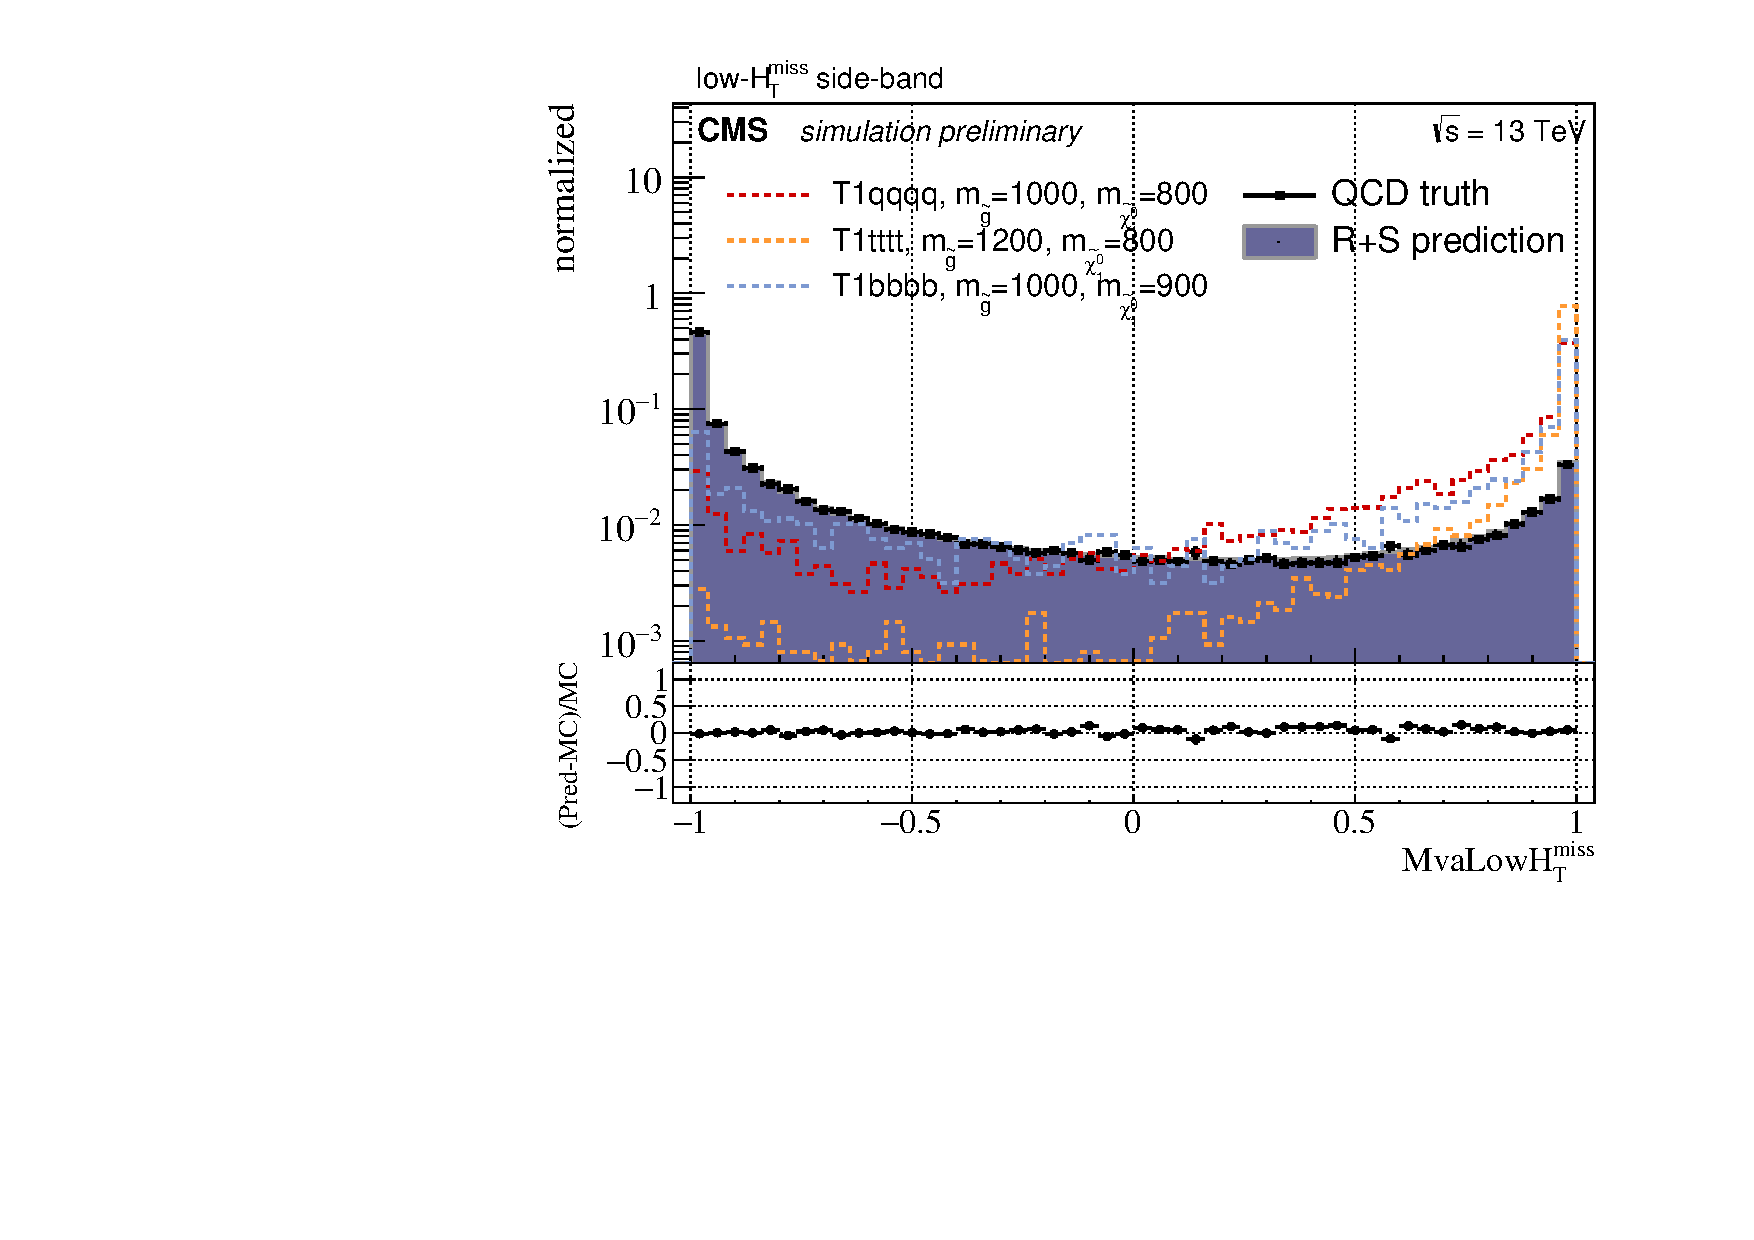
\includegraphics[width=0.7\linewidth]{figures/SusySearches/MvaSusy/MvaLowMht.pdf}
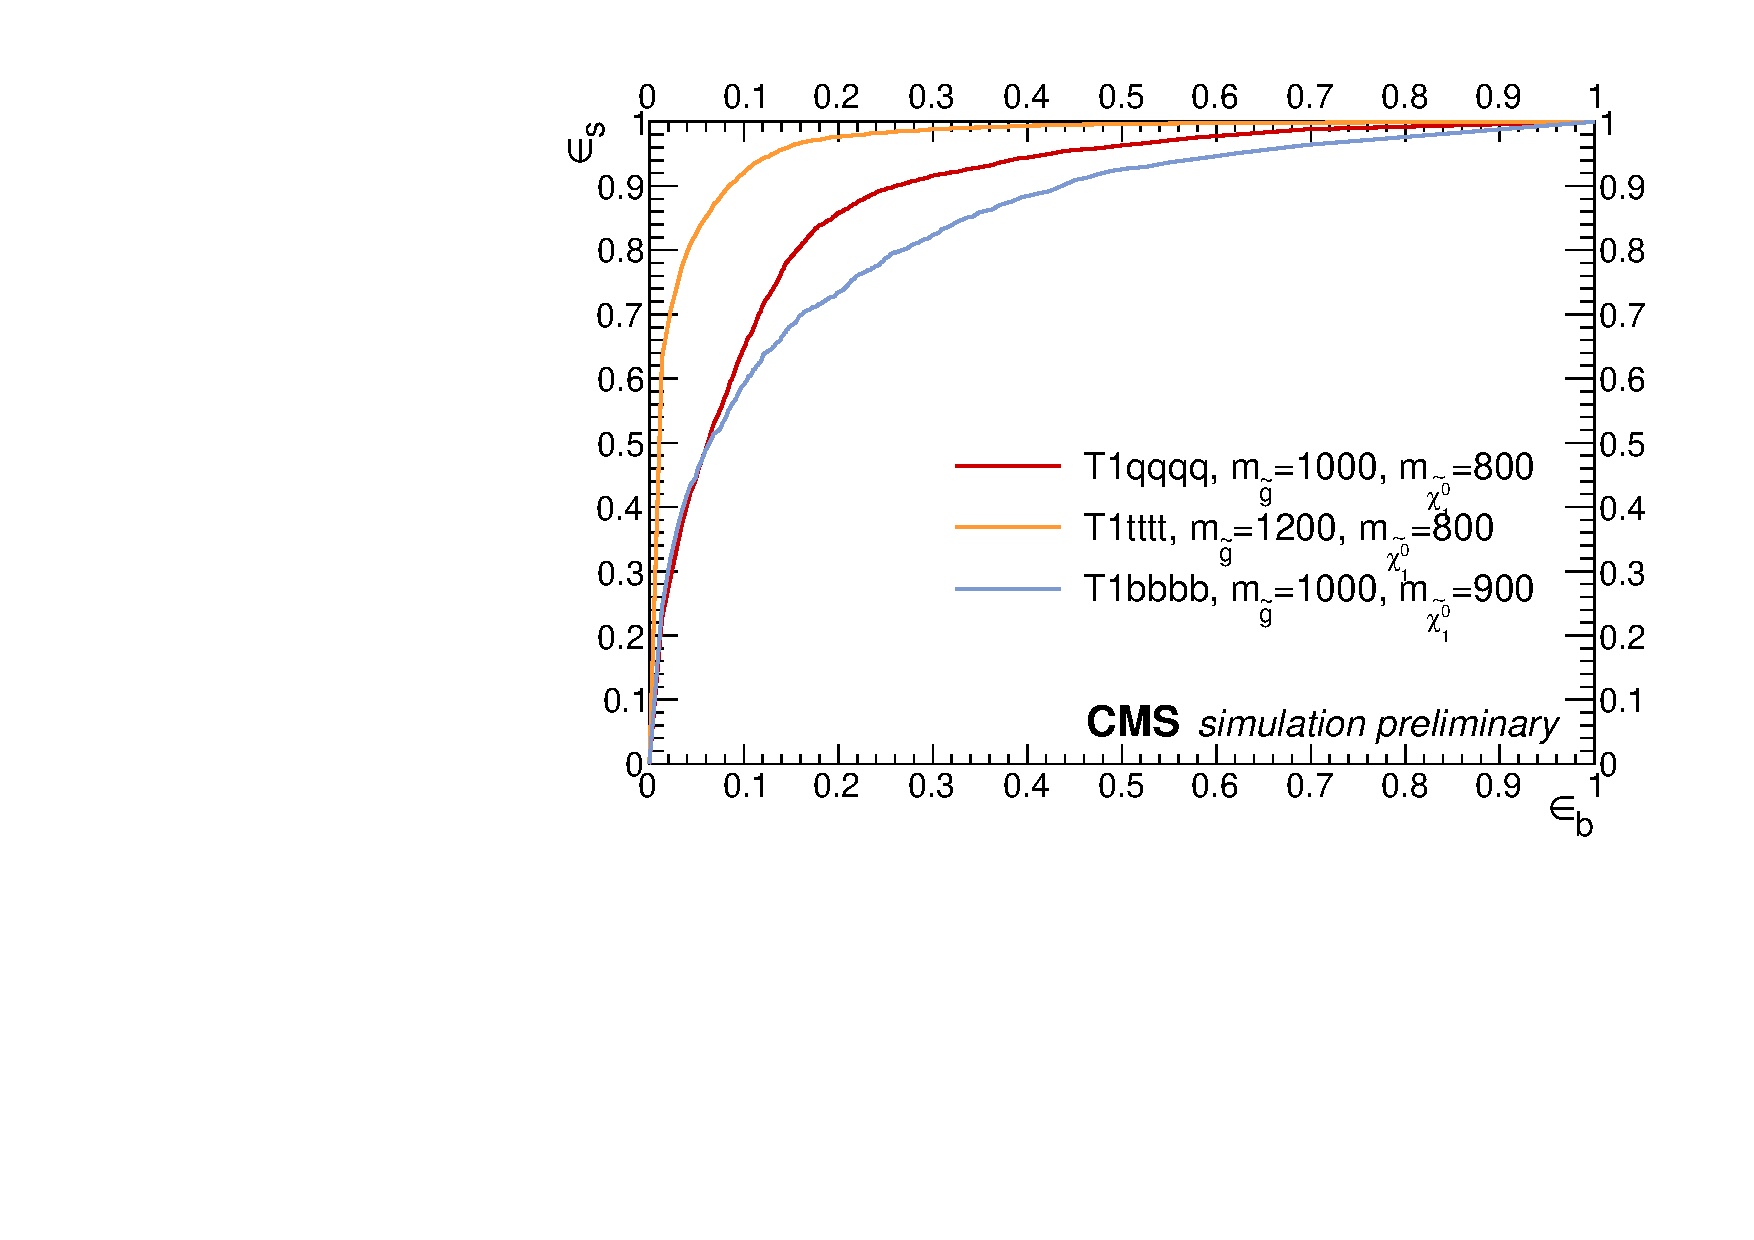
\includegraphics[width=0.7\linewidth]{figures/SusySearches/MvaSusy/RocCurvesLowMht_QCDVsSUSY.pdf}
\caption{Top: the distribution of the output of the low-$\mht$ data-driven discriminant for a sample of simulated QCD events, compared with the distribution obtained by applying the rebalance and smear method to simulation. Also shown are the distributions of the output for a few signal points corresponding to various SMS scenarios. Bottom: the efficiency of selecting signal events as a function of the efficiency for selecting background events, based on a scan through all possible thresholds on the discriminant.}
\label{fig:SusyBdt}
\end{figure}

\subsection{Low-$\Ht$ discriminant}
\label{sec:chosentarget}
A similar procedure is applied in the low-$\Ht$ signal region. In this region, the dominant standard model background is from the production of $Z$ bosons in association with jets, where the $Z$ decays into neutrinos. Therefore, I focus on rejecting $\zinv$ events while accepting SUSY signal events with high efficiency. Using the data-driven $\zinv$ background estimation methods described in Section \ref{sec:zinv}, and continuing the approach of using real data samples for the background training events for multivariate discriminants, the following strategy is used.
\begin{itemize}
\item Obtain a $\zinv$ prediction sample based on a real sample of $\zmumu$ events that have been cleaned of muons using the procedure described in Section \ref{sec:zinv};
\item use the same samples of SUSY signal events considered for the low-$\mht$ exercise;
\item train a BDT using the $\zinv$ prediction sample for the background events, and the pooled events from the SUSY model points for the signal events;
\item observe the accuracy of the modeling of the discriminant output by comparing the data-driven prediction applied in simulation using dielectron sample with the output obtained directly from $\zinv$ simulation, and
\item observe potential sensitivity to the signal models.
\end{itemize}
The modeling of the discriminant distribution for a simulated sample of $\zinv$ events is shown in Fig. \ref{fig:SusyBdt2}, along with the distribution for the sample obtained by applying the dielectron prediction method to $\zee$ simulation. Overlaid are distributions of the chosen signal model points. Once again, significant sensitivity gains are achieved across a range of SUSY models, and the discriminant is accurately modeled by the data-driven method developed herein. 
\begin{figure}[tb!]
\centering
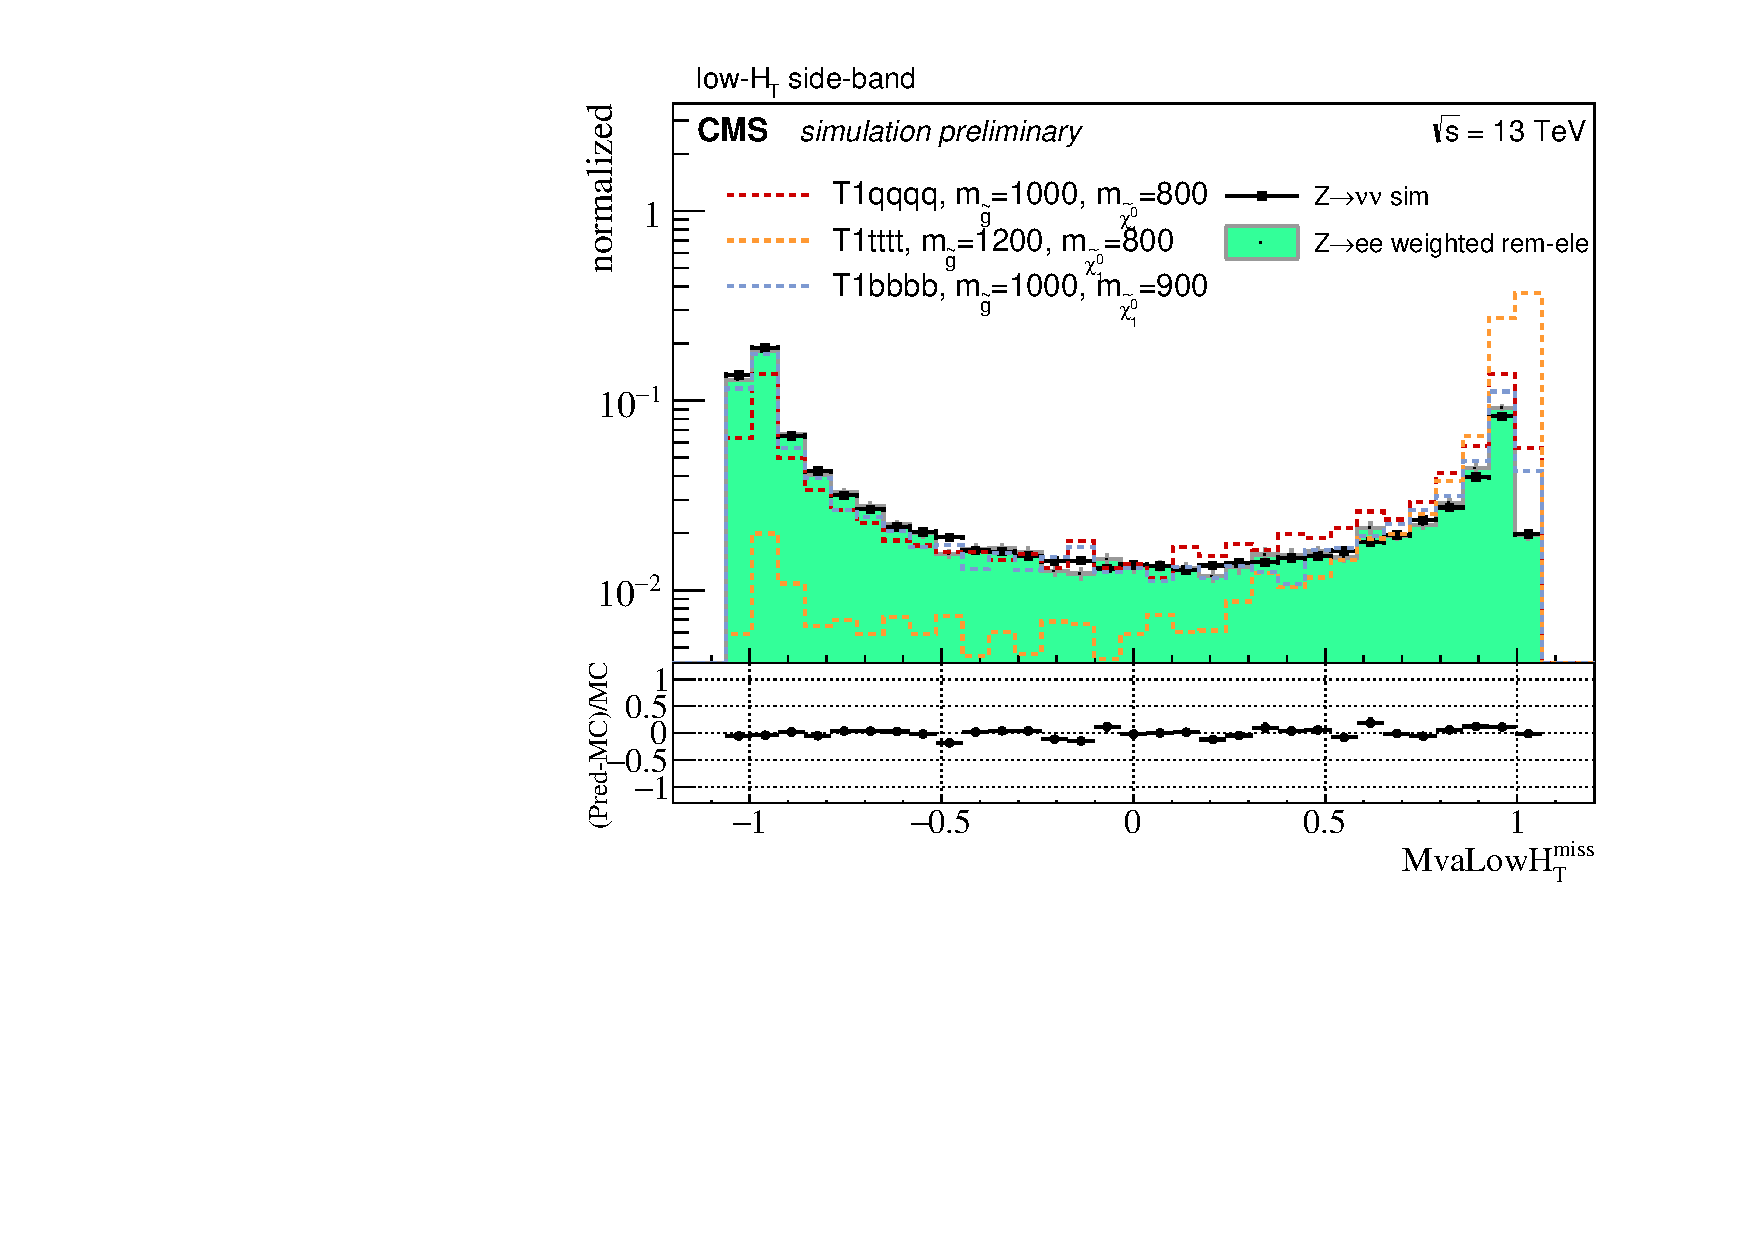
\includegraphics[width=0.7\linewidth]{figures/SusySearches/MvaSusy/MvaLowHt.pdf}
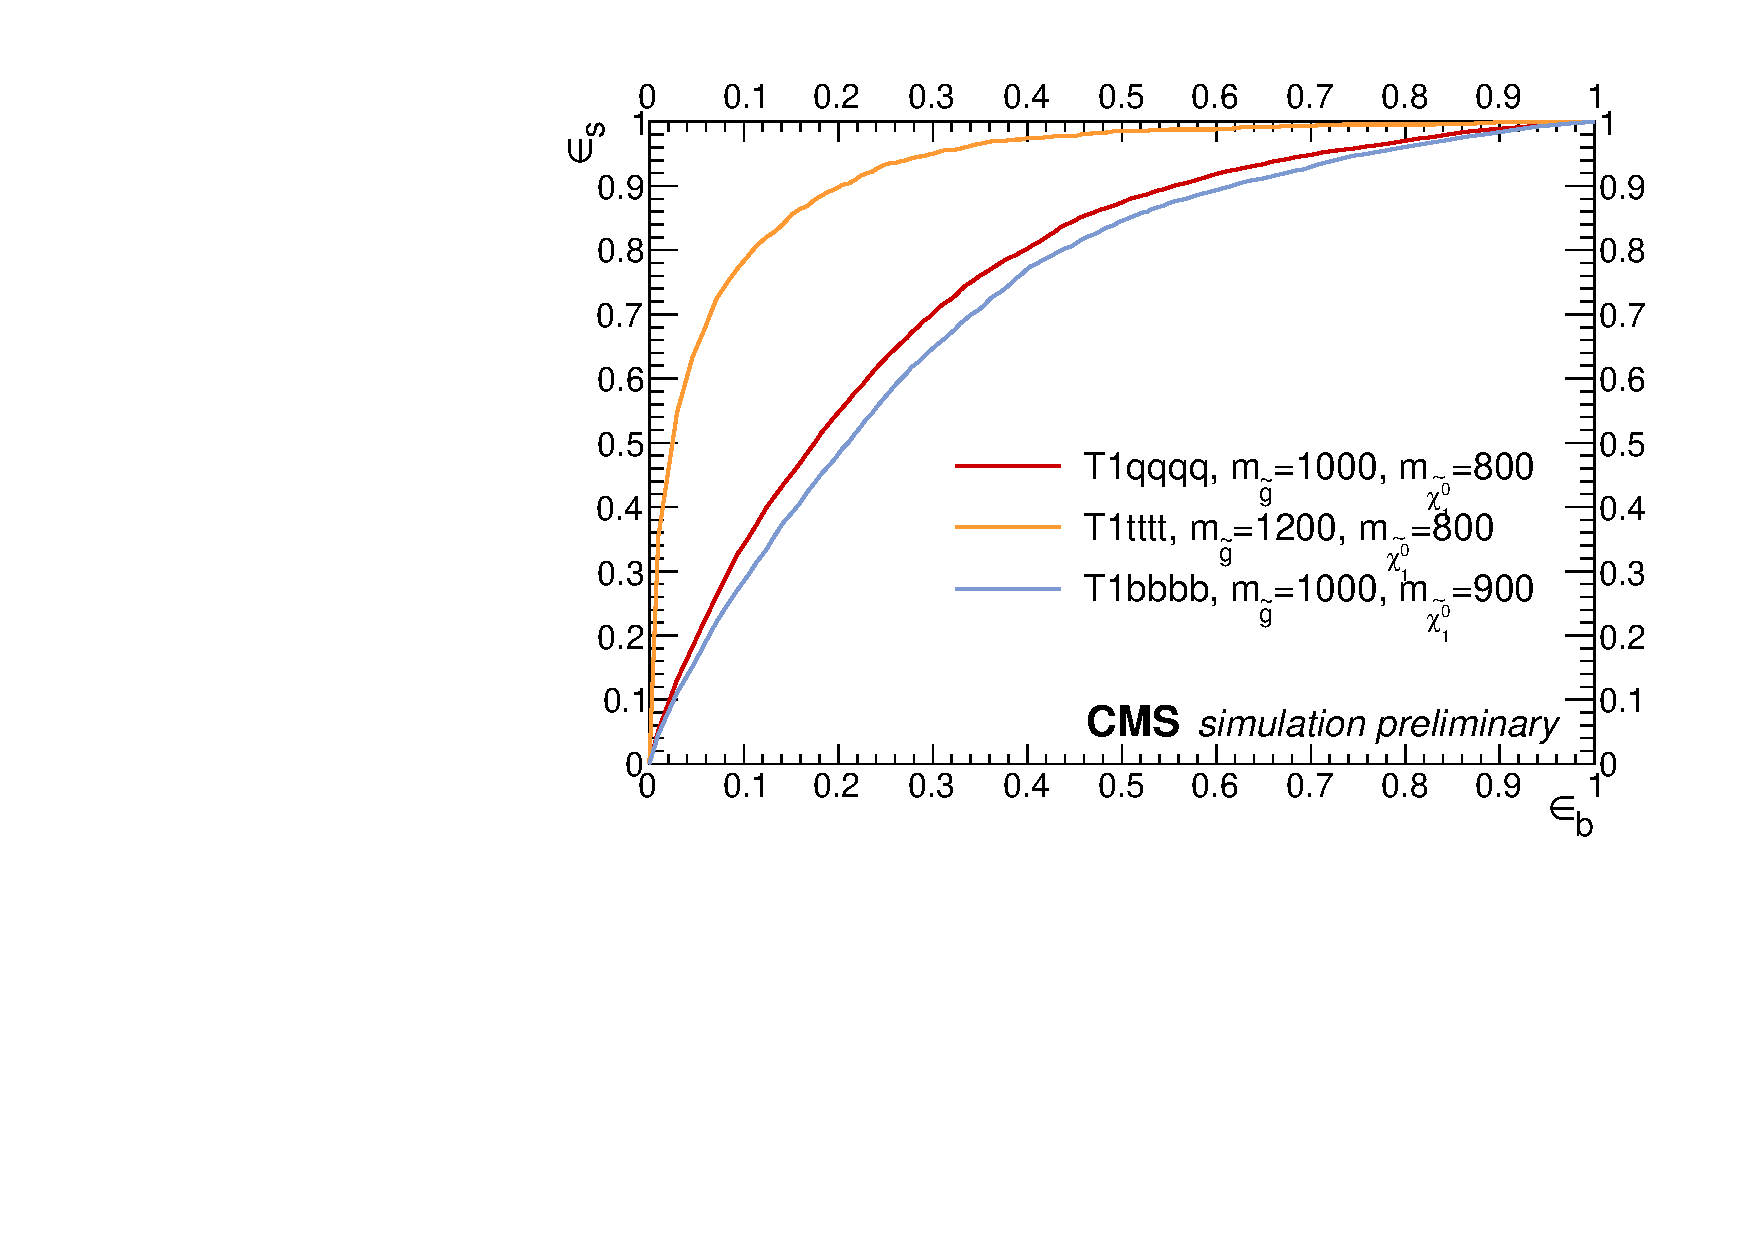
\includegraphics[width=0.7\linewidth]{figures/SusySearches/MvaSusy/RocCurvesLowHt_ZinvVsSUSY.pdf}
\caption{Top: The distribution of the output of the low-$\Ht$ muon data-driven multivariate discriminant for a sample of simulated $\zinv$ events, compared with the distribution obtained by applying the data-driven dielectron prediction method to simulation. Also shown are the distributions of the output for a few signal points corresponding to various SMS scenarios. Bottom: the efficiency of selecting signal events vs that of selecting background events, based on a scan through all possible thresholds on the discriminant.}
\label{fig:SusyBdt2}
\end{figure}

\section{Proof of principle analysis}
\label{sec:lastbattle}
As a proof of principle, I now present an analysis that follows the second approach described in Section \ref{sec:chosentarget}. Rather than targeting signal events corresponding to SMS models, however, the non-excluded regions of the pMSSM are used to design the search. A benchmark pMSSM point is chosen where the gluino and LSP masses are 644 and 400 GeV, respectively. The principal physics process corresponding to this point is that shown in Fig. \ref{fig:diagrams2} (b), in which gluinos are pair produced, each gluino decays into a q$\bar{\text{q}}$ pair and a 400 GeV chargino, and the chargino decays into a W boson and an LSP. This model point survived the run 1 CMS searches, and is referred to as survivor 1 in the figures. Fig. \ref{fig:Survivors} shows distributions of key observables predicted by the benchmark signal scenario, normalized to a luminosity of 2.3 fb$^{-1}$. 
\begin{figure}[tb!]
\centering
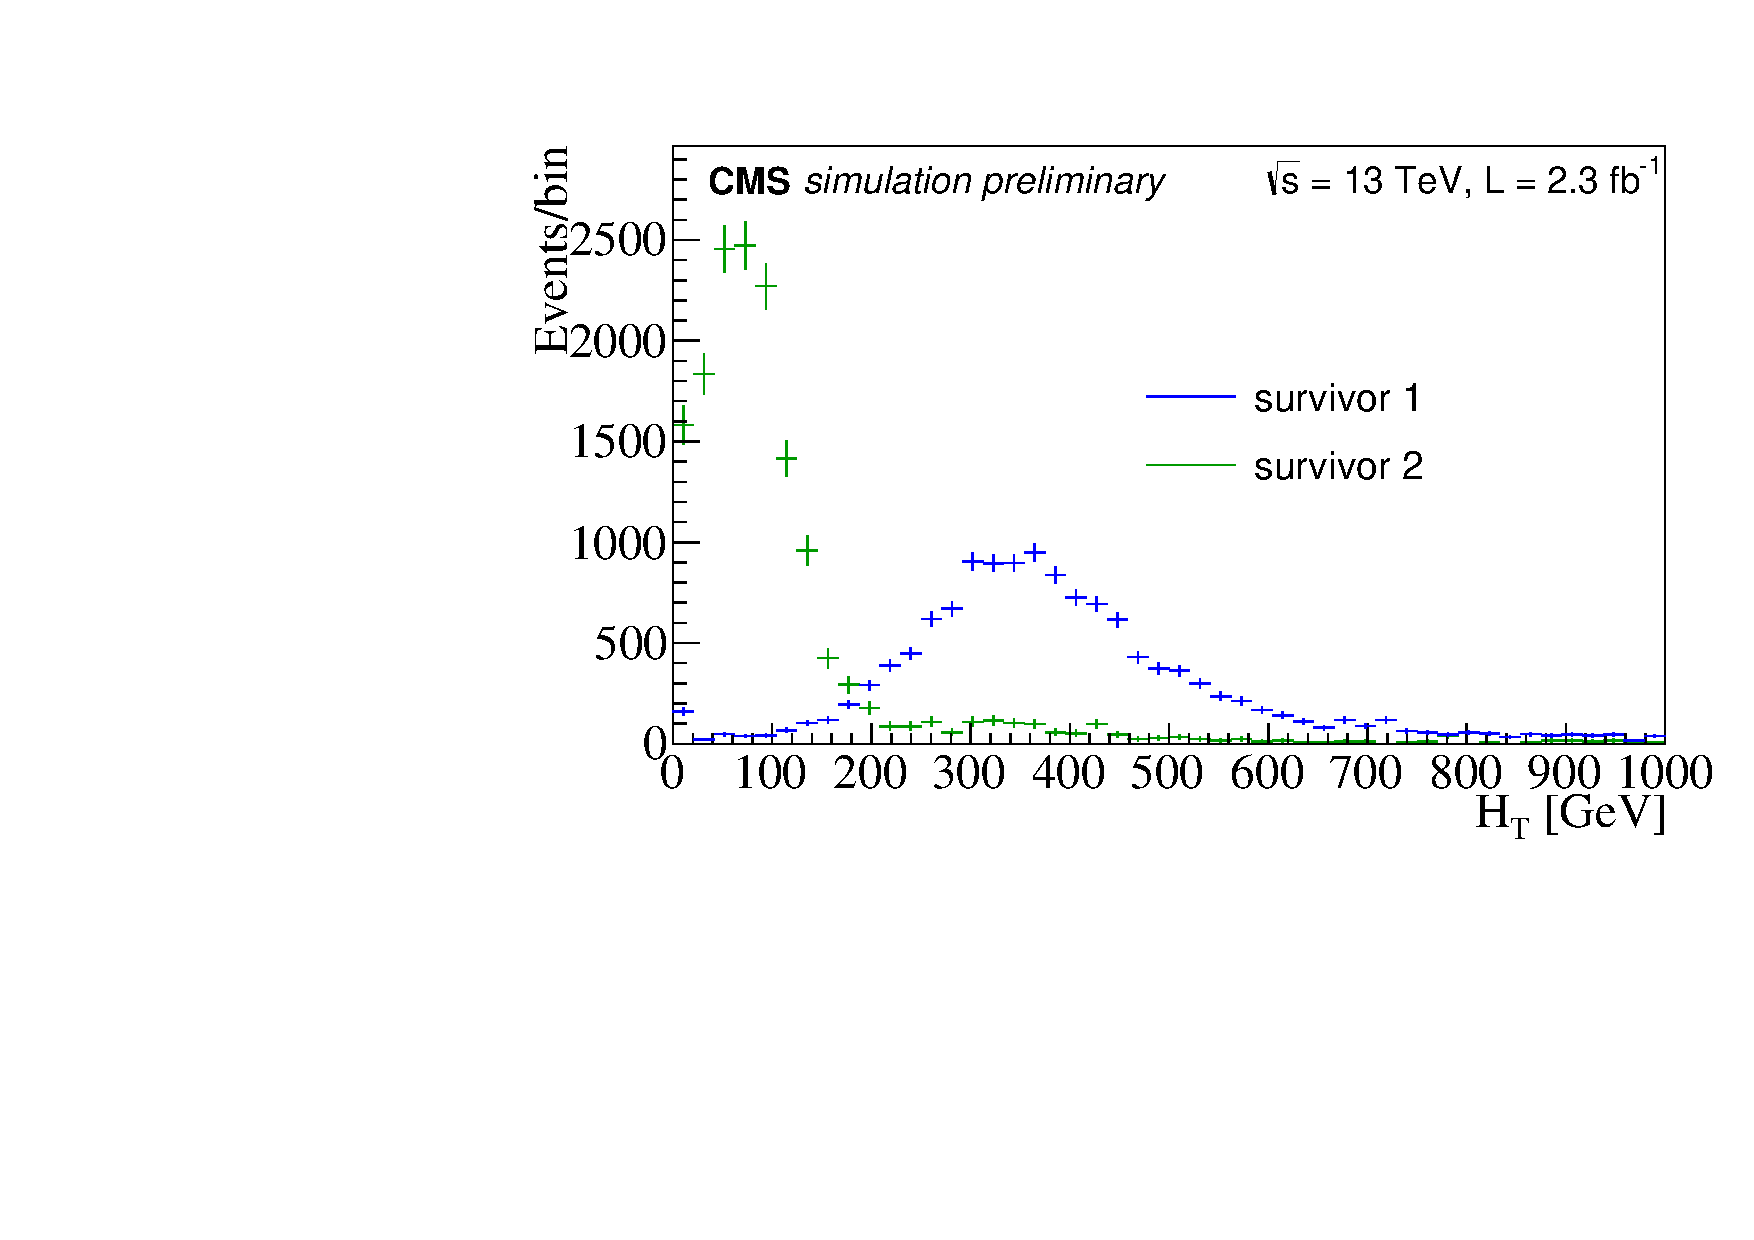
\includegraphics[width=0.45\linewidth]{figures/SusySearches/MvaSusy/SurvivorsHt.pdf}
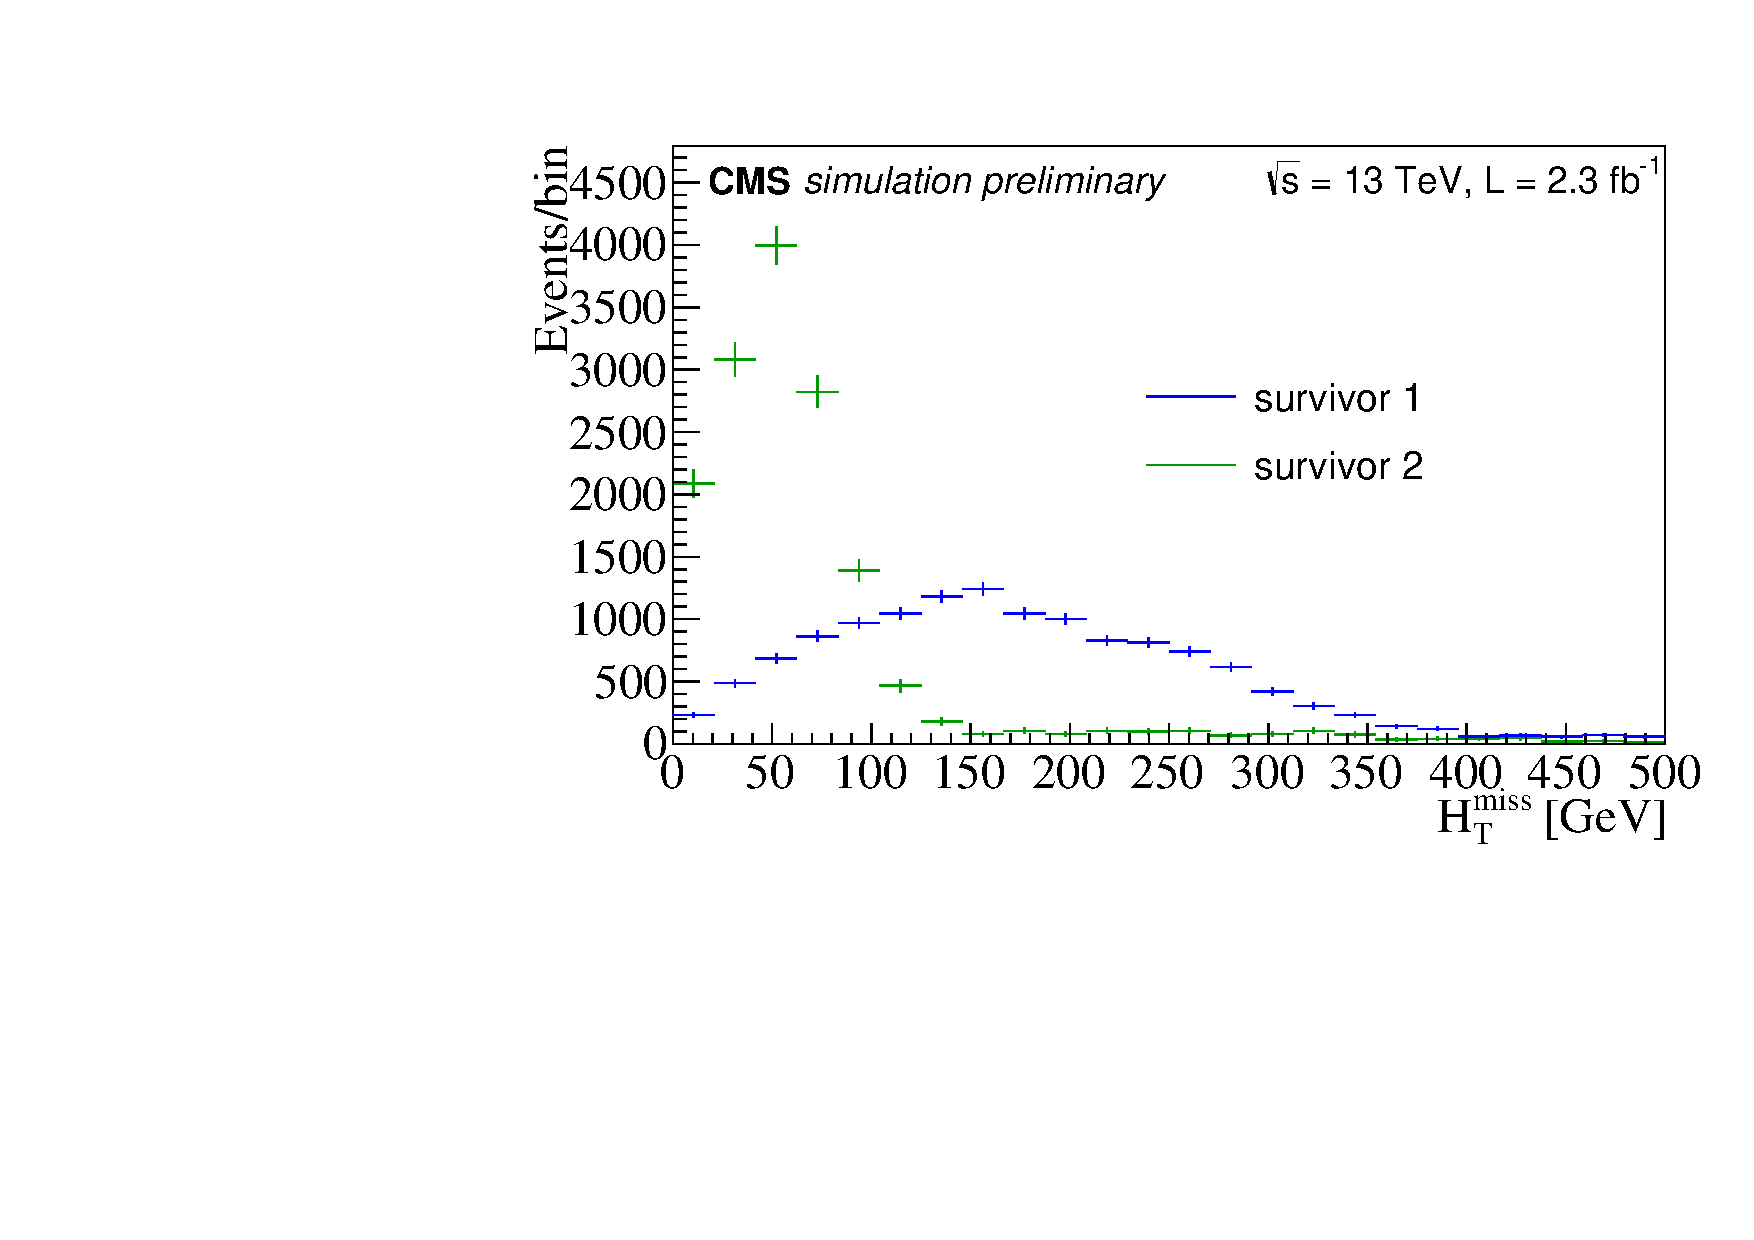
\includegraphics[width=0.45\linewidth]{figures/SusySearches/MvaSusy/SurvivorsMht.pdf}
\caption{Kinematic distributions of selected low-mass gluino pMSSM points. The benchmark pMSSM point, referred to as survivor 1, is shown in blue.}
\label{fig:Survivors}
\end{figure}
The $\Ht$ distribution, which peaks at 350 GeV, illuminates why this model was not excluded in run 1. The 7 and 8 TeV hadronic analyses imposed a threshold of 500 GeV on the $\Ht$ as part of the baseline selection. I note that the same selection is applied in the 13 TeV hadronic searches, which likely have also not excluded this point. 

Figure \ref{fig:Survivors} suggests that a good choice of signal region is a low-$\Ht$ sideband of the CMS multi-jet $+$ $\mht$ search \cite{Khachatryan:2016kdk}. I choose a baseline selection:
\begin{itemize}
\item $400<\Ht<500$ GeV;
\item $\mht>200$ GeV;
\item $\njets\geq$ 4, where jets are required to have a $\pt>30$ GeV and $|\eta|<2.4$, and
\item $\Delta\phi(\mht$, jet$_{1,2,3,4})>$ 0.5, 0.5, 0.3, 0.3,
\end{itemize}
which applies to all control regions and the signal baseline region. Events in the signal baseline region are further required to satisfy 
\begin{itemize}
\item $N_{\text{lep}}=0$, with lepton $\pt>10$ GeV and $|\eta|<2.4$, and isolation defined analogously with  \cite{Khachatryan:2016kdk};
\item $\nbjets=0$.
\end{itemize}

Events are collected using the monojet trigger featured in Section \ref{sec:hadronictrigger}. Events are required to have both an online $\mht$ and $\met$ in excess of 90 GeV. Because there is no online threshold on the $\Ht$, events satisfying the baseline selection are accepted by the monojet trigger with nearly 100\% probability.

A BDT is trained using events from excluded pMSSM points for the signal training sample, and a set of $\zinv$ proxy events for the background training sample, where the proxy events are those used to train the BDT in the previous section. Approximately 27,000 signal events and 6,000 background events are used in the training, choices dictated by the availability of events. The 15 inputs to the BDT are the $\mht$, $\phi^{\text{miss}}$, $\Ht$, $\njets$, and the $\pt$, $\eta$, and $\phi$ of the four leading jets in an event, and the output is a single-valued discriminant. The discriminant ranges from $-1$ to $1$, where $-1$ corresponds to more background-like events, and $+1$ to more signal-like events. The range is divided evenly into 10 bins. The left-most bin is seen to receive a negligible contribution from the signal, and so is used as a normalization control region. The left 9 bins are designated as signal regions labeled, from left to right, ``SR1'',..., ``SR9''.

The principal sources of background events are those of the multi-jet $+$ $\mht$ search \cite{Khachatryan:2016kdk}. These include events in which a Z boson is produced and decays into neutrinos ($\zinv$), events in which jets are produced in association with a W boson that decays into leptons that are not identified (W$+$jets), events in which a top quark pair is produced in association with jets and final-state leptons are not identified (t$\bar{\text{t}}$), and QCD multi-jets events. Given that the BDT is sensitive to the correlations among the 15 input observables, it is advantageous to carry out a fully data driven background prediction. The estimation procedure is described below.

\subsection{Backgrounds}
Predictions for the $\zinv$ and QCD counts in the signal regions are readily carried out using the rebalance and smear and dilepton cleaning methods, respectively. Uncertainties in the QCD estimates are obtained using the procedure described in Section \ref{sec:qcd}. Uncertainties in the $\zinv$ prediction are statistical uncertainties associated with the two-electron control region, the residuals of the simulated closure test, and a 5\% systematic uncertainty associated with the efficiency maps, which are derived in simulation. The backgrounds of W$+$jets and t$\bar{\text{t}}$ are estimated using the following method. 

\subsubsection{Prediction for t$\bar{\text{t}}$ and W$+$jets}
Events arising from the signal benchmark scenario do not contain heavy flavor jets, that is, jets originating from bottom or top quarks, nor events with leptons. Therefore, a sample of real events having one or more b-tagged jet or one or more lepton is expected to comprise primarily t$\bar{\text{t}}$ and W$+$jets events, and no signal events. Because the only difference between t$\bar{\text{t}}$ events with 0 b-tags and those with 2 b-tags is whether or not the b-jets in the event are tagged as such, one expects the shape of the discriminant distribution of the 0 and 2 b-tag event sets to be similar. This is confirmed in simulation, as seen in Fig. \ref{fig:ttbar2b0b}, where the discriminant  distribution for t$\bar{\text{t}}$ events with 0 b-tags is compared with the same for events with 2 b-tags; it is found that the shapes agree within statistical uncertainties. This similarity motivates the use of a real 2 b-tag data sample to define the t$\bar{\text{t}}$ template.
\begin{figure}[tb!]
\centering
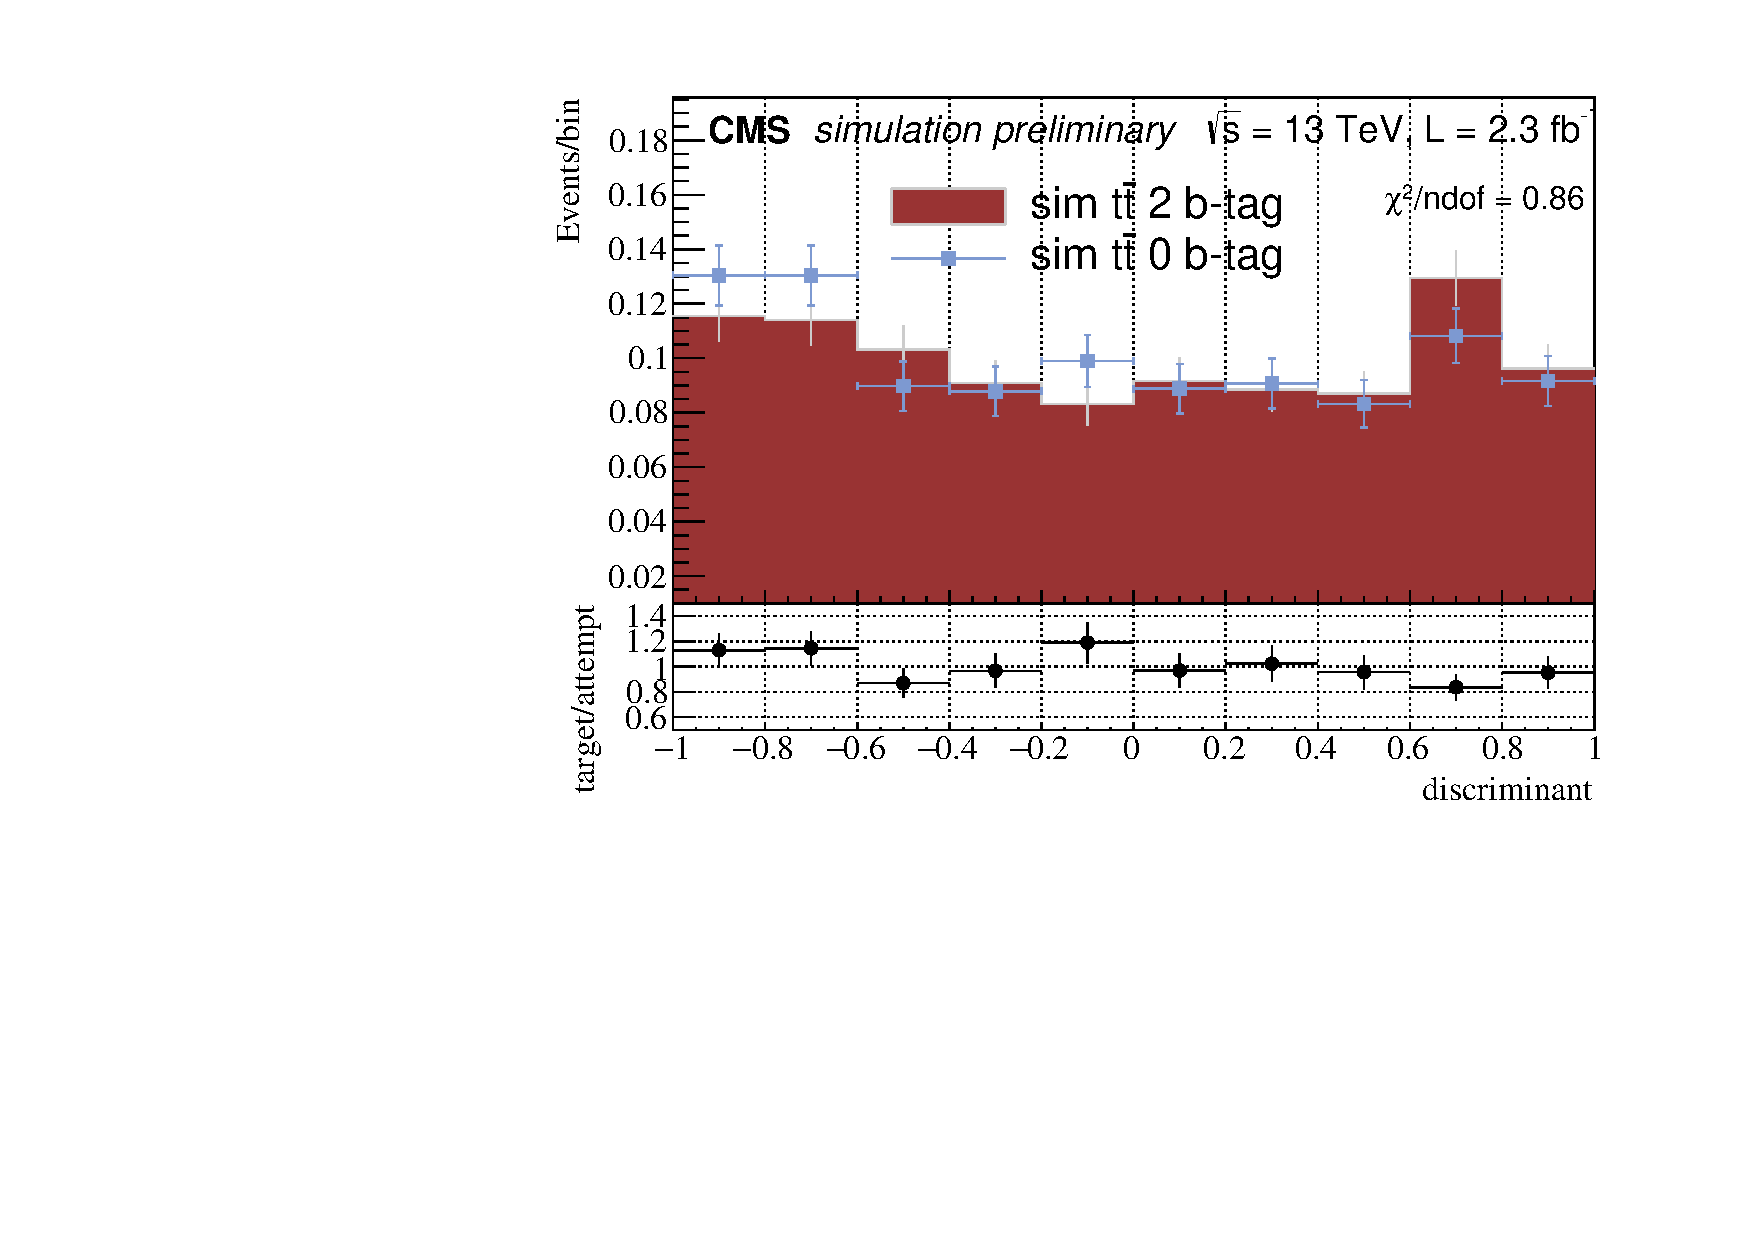
\includegraphics[width=0.55\linewidth]{figures/SusySearches/MvaSusy/TTbar2bVs0b.pdf}
\caption{Comparison of the normalized discriminant between simulated t$\bar{\text{t}}$ events with 2 b-tags and 0 b-tags, in the baseline region.}
\label{fig:ttbar2b0b}
\end{figure}

Simulation also reveals that W$+$jets events yield a discriminant distribution that is indistinguishable from that of t$\bar{\text{t}}$ events (Figure \ref{fig:ttbarVsWjets}).
\begin{figure}[tb!]
\centering
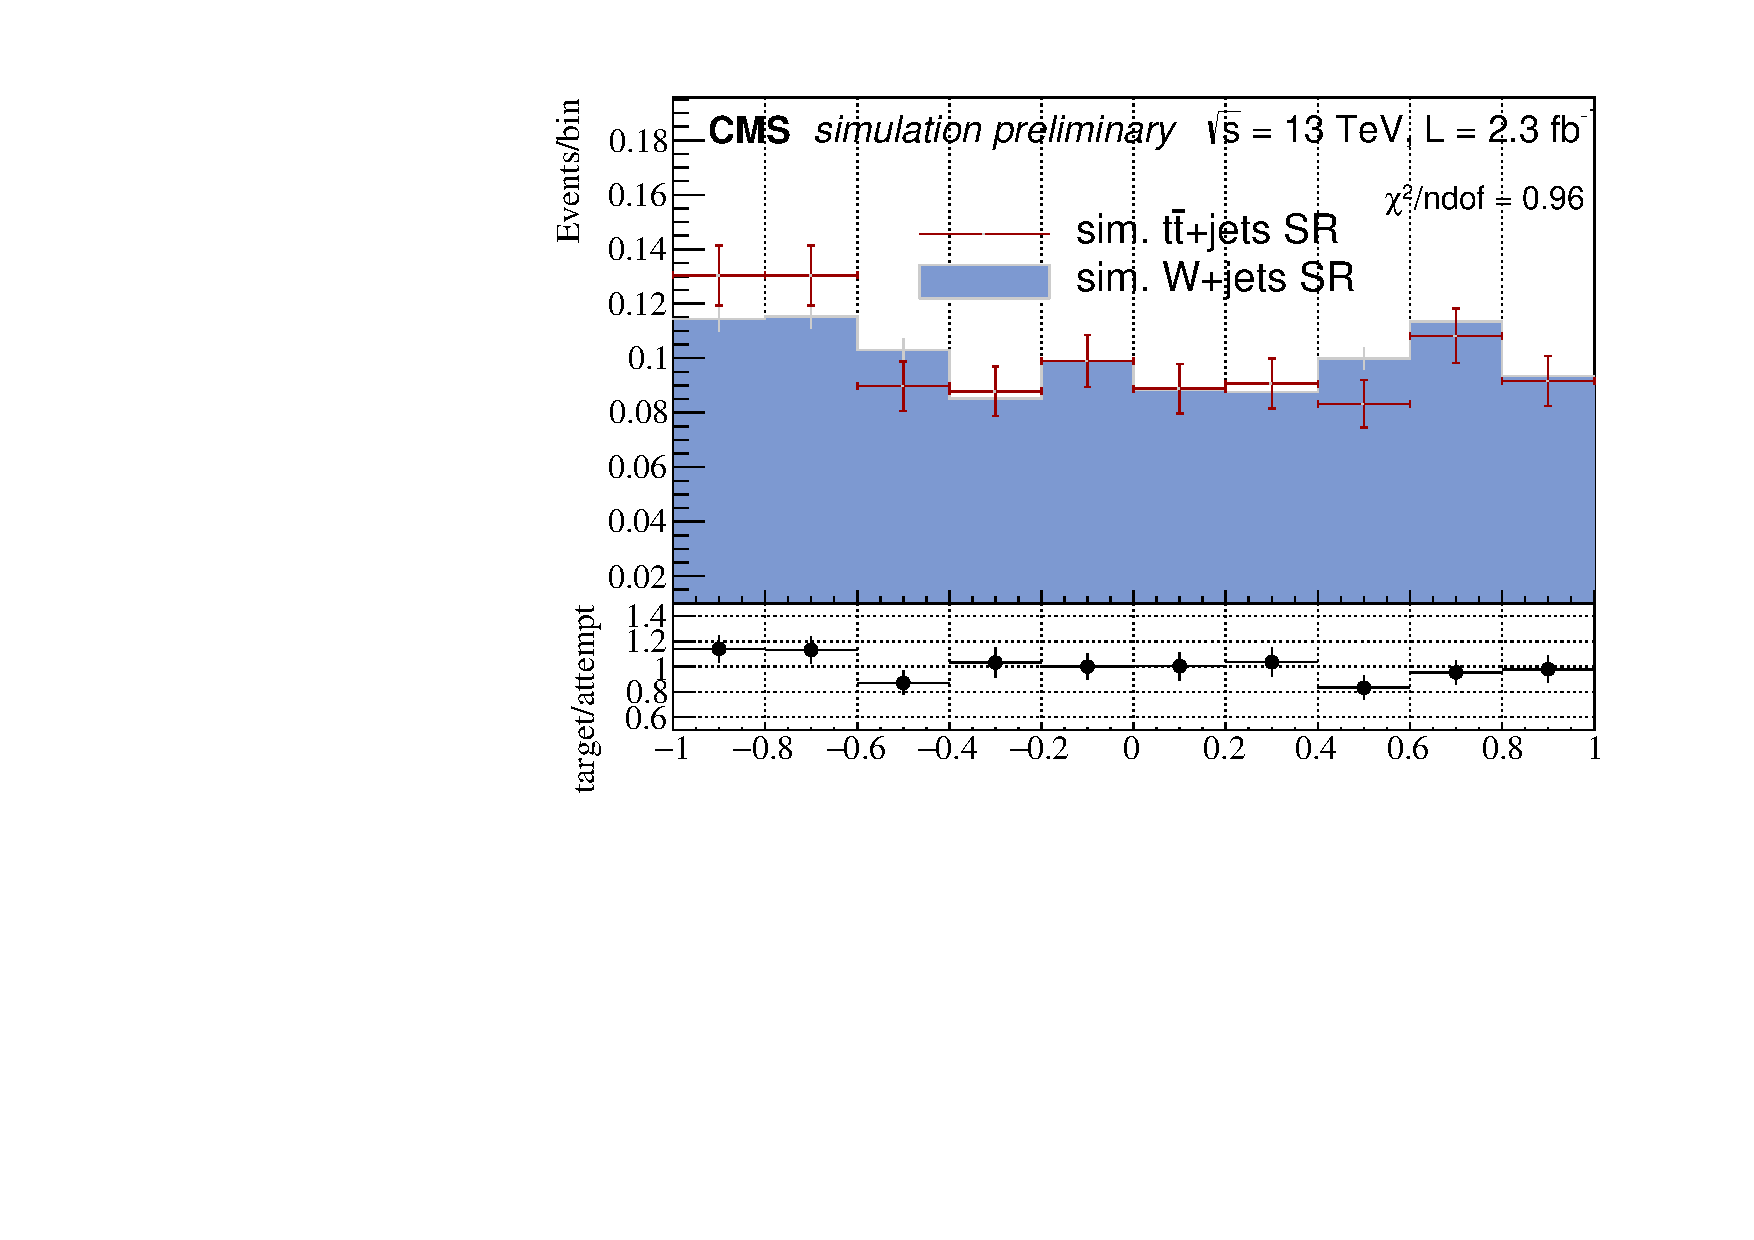
\includegraphics[width=0.55\linewidth]{figures/SusySearches/MvaSusy/TTWSimCompare.pdf}
\caption{Comparison of the normalized discriminant between simulated t$\bar{\text{t}}$ events and W$+$jets events, in the signal baseline region.}
\label{fig:ttbarVsWjets}
\end{figure}
Furthermore, simulation indicates that the shapes of the output of the discriminant in the baseline region are indistinguishable across a range of final states, among them final states with 0, 1, and 2 b-tagged jets, as well as final states with 0 and 1 lepton, for both t$\bar{\text{t}}$ events and W$+$jets events. Therefore, real data samples corresponding to these final states are used to derive shape templates for the combined contribution from t$\bar{\text{t}}$ events and W$+$jets backgrounds. The similarity of the shapes for the two backgrounds is checked in real data by comparing samples with various relative contributions from t$\bar{\text{t}}$ and W$+$jets. These regions include the 2 b-tag 0-lepton region, the 0 b-tag 1-lepton region, and regions with various numbers of b-tags and leptons. Shapes of distributions defined with the above sets of selection are seen to be compatible in Fig. \ref{fig:data2b0lVs1b1l}.
\begin{figure}[tb!]
\centering
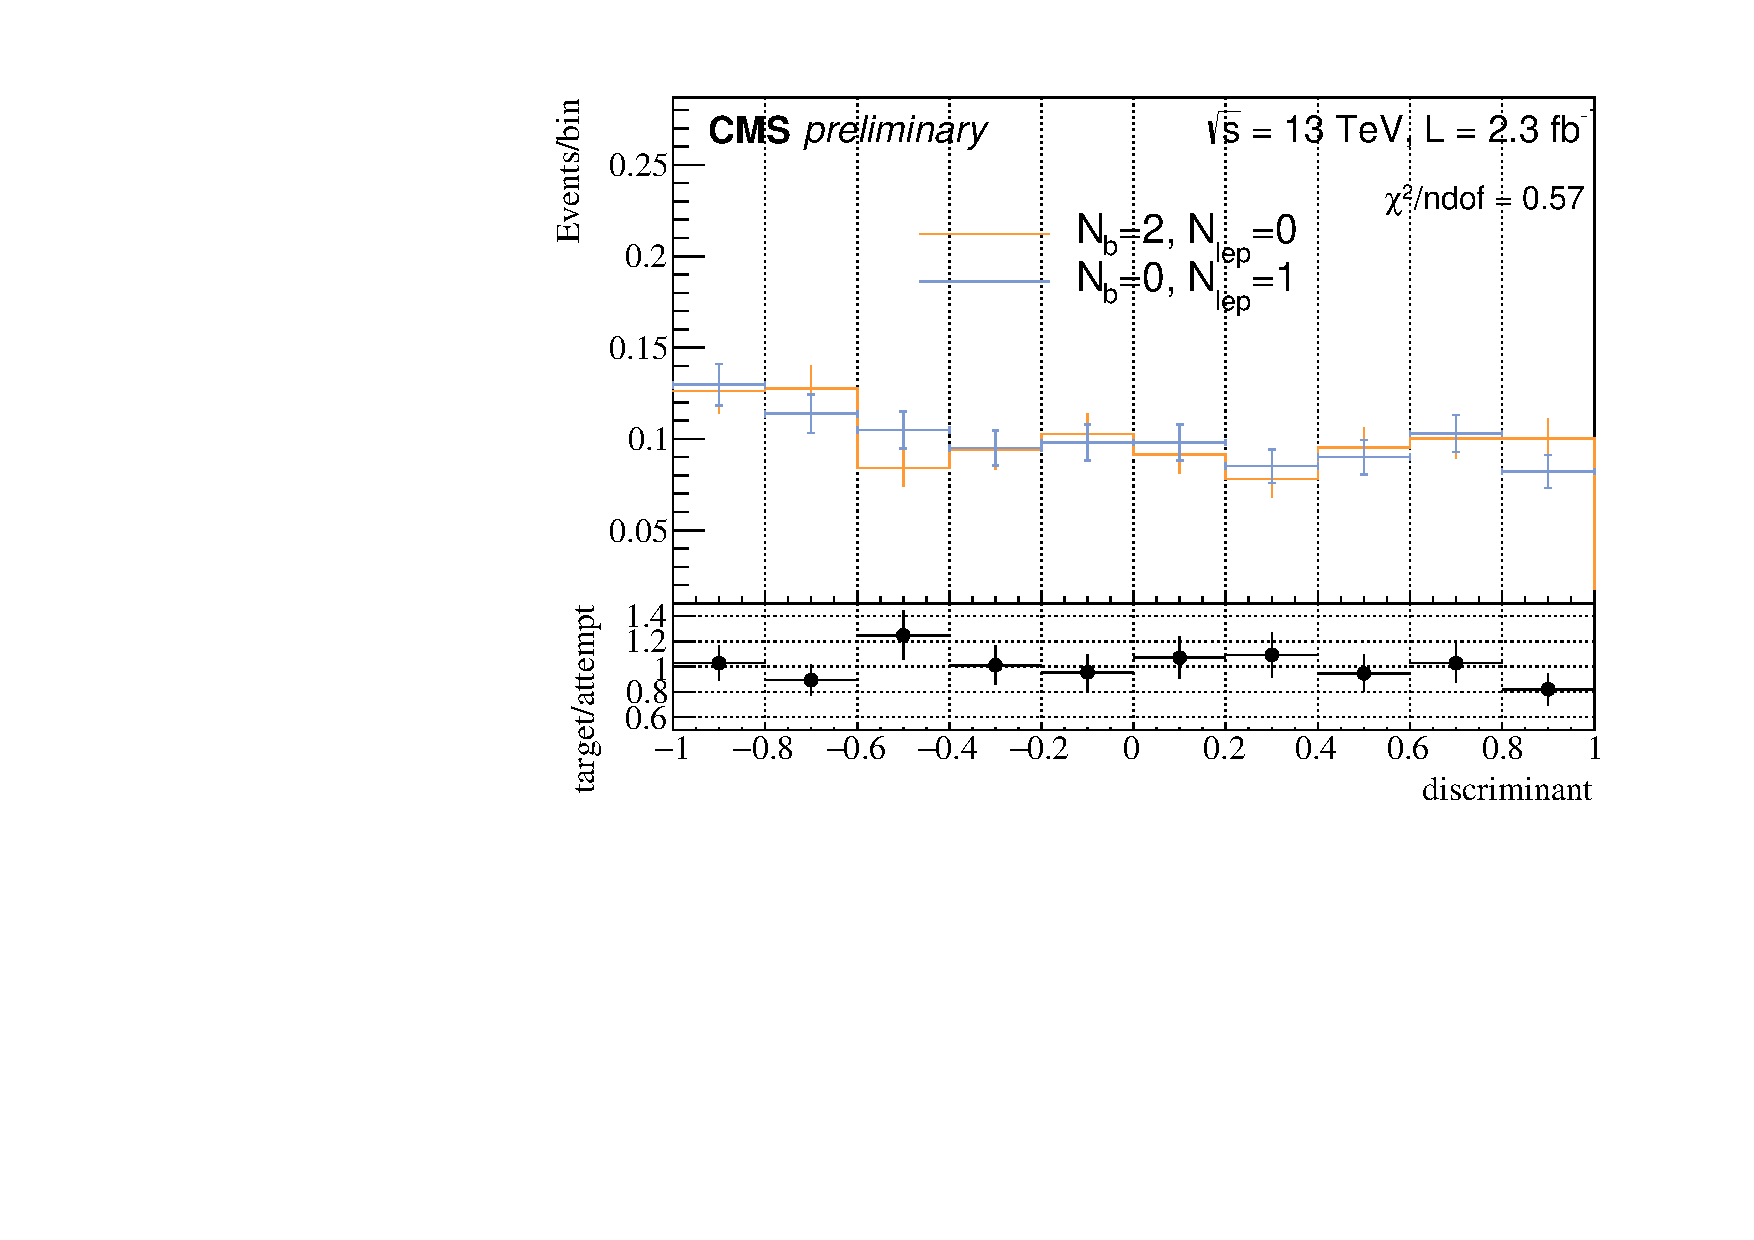
\includegraphics[width=0.55\linewidth]{figures/SusySearches/MvaSusy/Data_2b0Lvs0b1L.pdf}
\caption{Comparison of the output of the discriminant shapes in real data between control regions with various relative contributions from t$\bar{\text{t}}$ and W$+$jets events.}
\label{fig:data2b0lVs1b1l}
\end{figure}

The t$\bar{\text{t}}$/W$+$jets shape template and associated uncertainty is derived from the pooled b-tag and lepton control regions discussed above. The normalization of the  t$\bar{\text{t}}$/W$+$jets template is fixed by the observed count in the normalization control region (the leftmost bin of the discriminant), less the predicted count from the other backgrounds in the normalization control region, namely, the leftmost bin of the discriminant. 
Given this choice of normalization, the predicted t$\bar{\text{t}}$ and W$+$jets event counts in the signal regions are anti-correlated with the prediction for the other backgrounds in the normalization control region. This anti-correlation is taken into account in the final prediction by generating ensembles of background predictions, where each prediction in the ensemble receives the full treatment described above, but has a unique value for the normalization obtained from a random sampling of a gaussian whose mean and standard deviation is the predicted count and uncertainty from non-t$\bar{\text{t}}$ and W$+$jets in the normalization region. All uncertainties are propagated through the ensemble.

Other backgrounds from rare standard model processes include single-top quark production, two and three boson production, and make only a minor contribution to the total background. These backgrounds are simulated, and uncertainties of 100\% are assumed for the counts in all signal regions. The signal counts are estimated from a sample of simulated events generated by {\sc pythia} 8~\cite{Sjostrand:2006za} and processed with the CMS fast detector simulation program~\cite{Abdullin:2011zz}. Uncertainties reflect the uncertainty in the signal cross section of 13\% and statistical uncertainties in the event sample on the order of 10\%. An additional   uncertainty, guessed to be 20\%, is assigned to account for PDF, scale, and ISR uncertainties. These uncertainties have not been computed directly due to time constraints, and this treatment should be improved in future iterations of the analysis. 

\subsection{Results}
Estimates of the total background counts and uncertainties in the signal regions, along with the observed counts, are given in Table \ref{tab:results}.  
 \begin{table}[htb]
    \label{tab:preCMS}
        \caption{Expected and observed counts and uncertainties, along with the prediction for the signal yield.}
    \centering
    \vspace{1ex}
    \begin{tabular}{c|c|c|c}
    \hline
    signal & expected    & observed  & signal  \\
    region & bkg. count    & count   & count  \\
    \hline\hline
1 & $229\pm48$ & $172$ & $9\pm5$\\
2 & $159\pm39$ & $192$ & $18\pm8$\\
3 & $157\pm35$ & $161$ & $36\pm13$\\
4 & $128\pm31$ & $163$ & $41\pm14$\\
5 & $137\pm35$ & $137$ & $68\pm21$\\
6 & $167\pm40$ & $157$ & $57\pm18$\\
7 & $162\pm39$ & $164$ & $104\pm29$\\
8 & $167\pm36$ & $194$ & $118\pm33$\\
9 & $127\pm30$ & $191$ & $61\pm19$\\
\hline
    \end{tabular}
    \label{tab:results}
    \end{table}
The full results are also shown in Fig. \ref{fig:results}, with the distribution of the benchmark pMSSM point included in the background stack. The results based on pure simulation are also shown for comparison, although are not used in the interpretation. 
\begin{figure}[tb!]
\centering
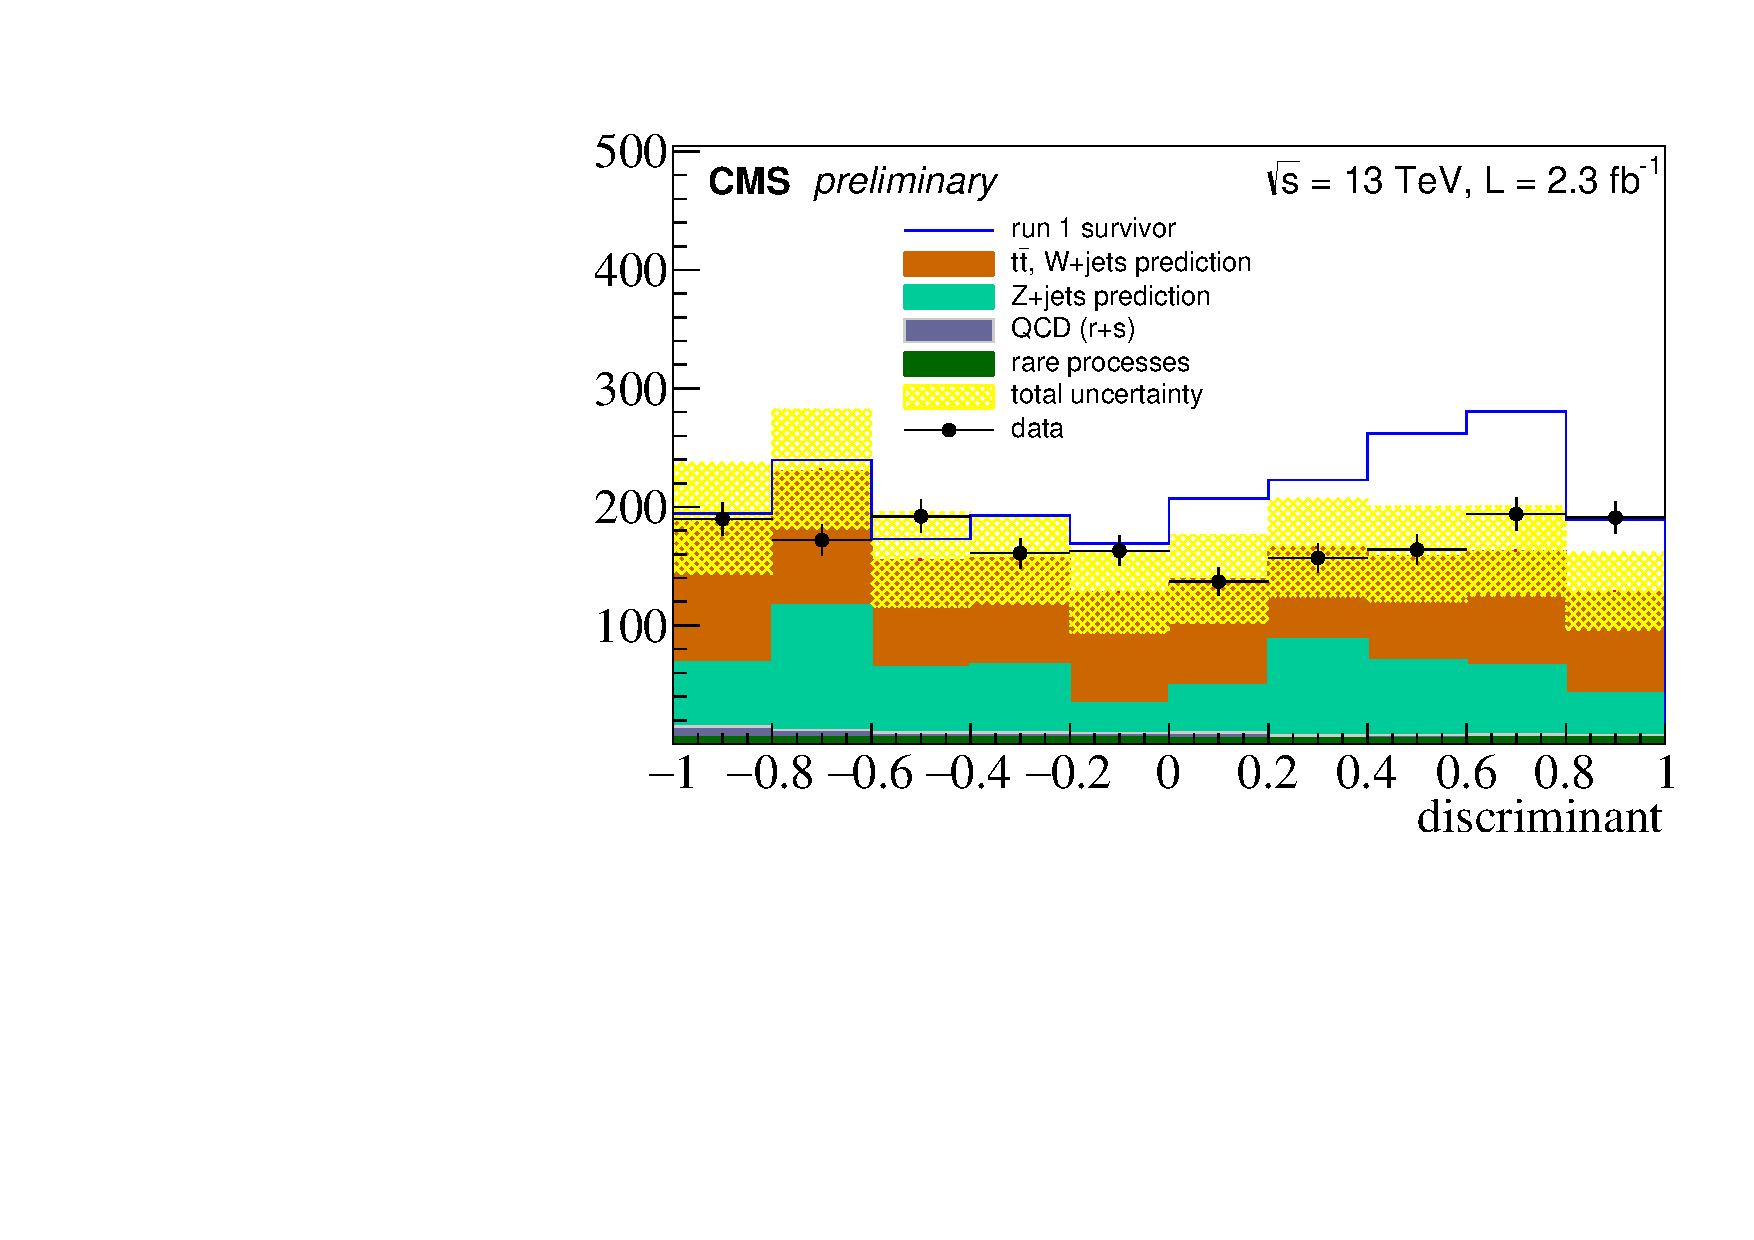
\includegraphics[width=0.65\linewidth]{figures/SusySearches/MvaSusy/ResultDD.pdf}\\
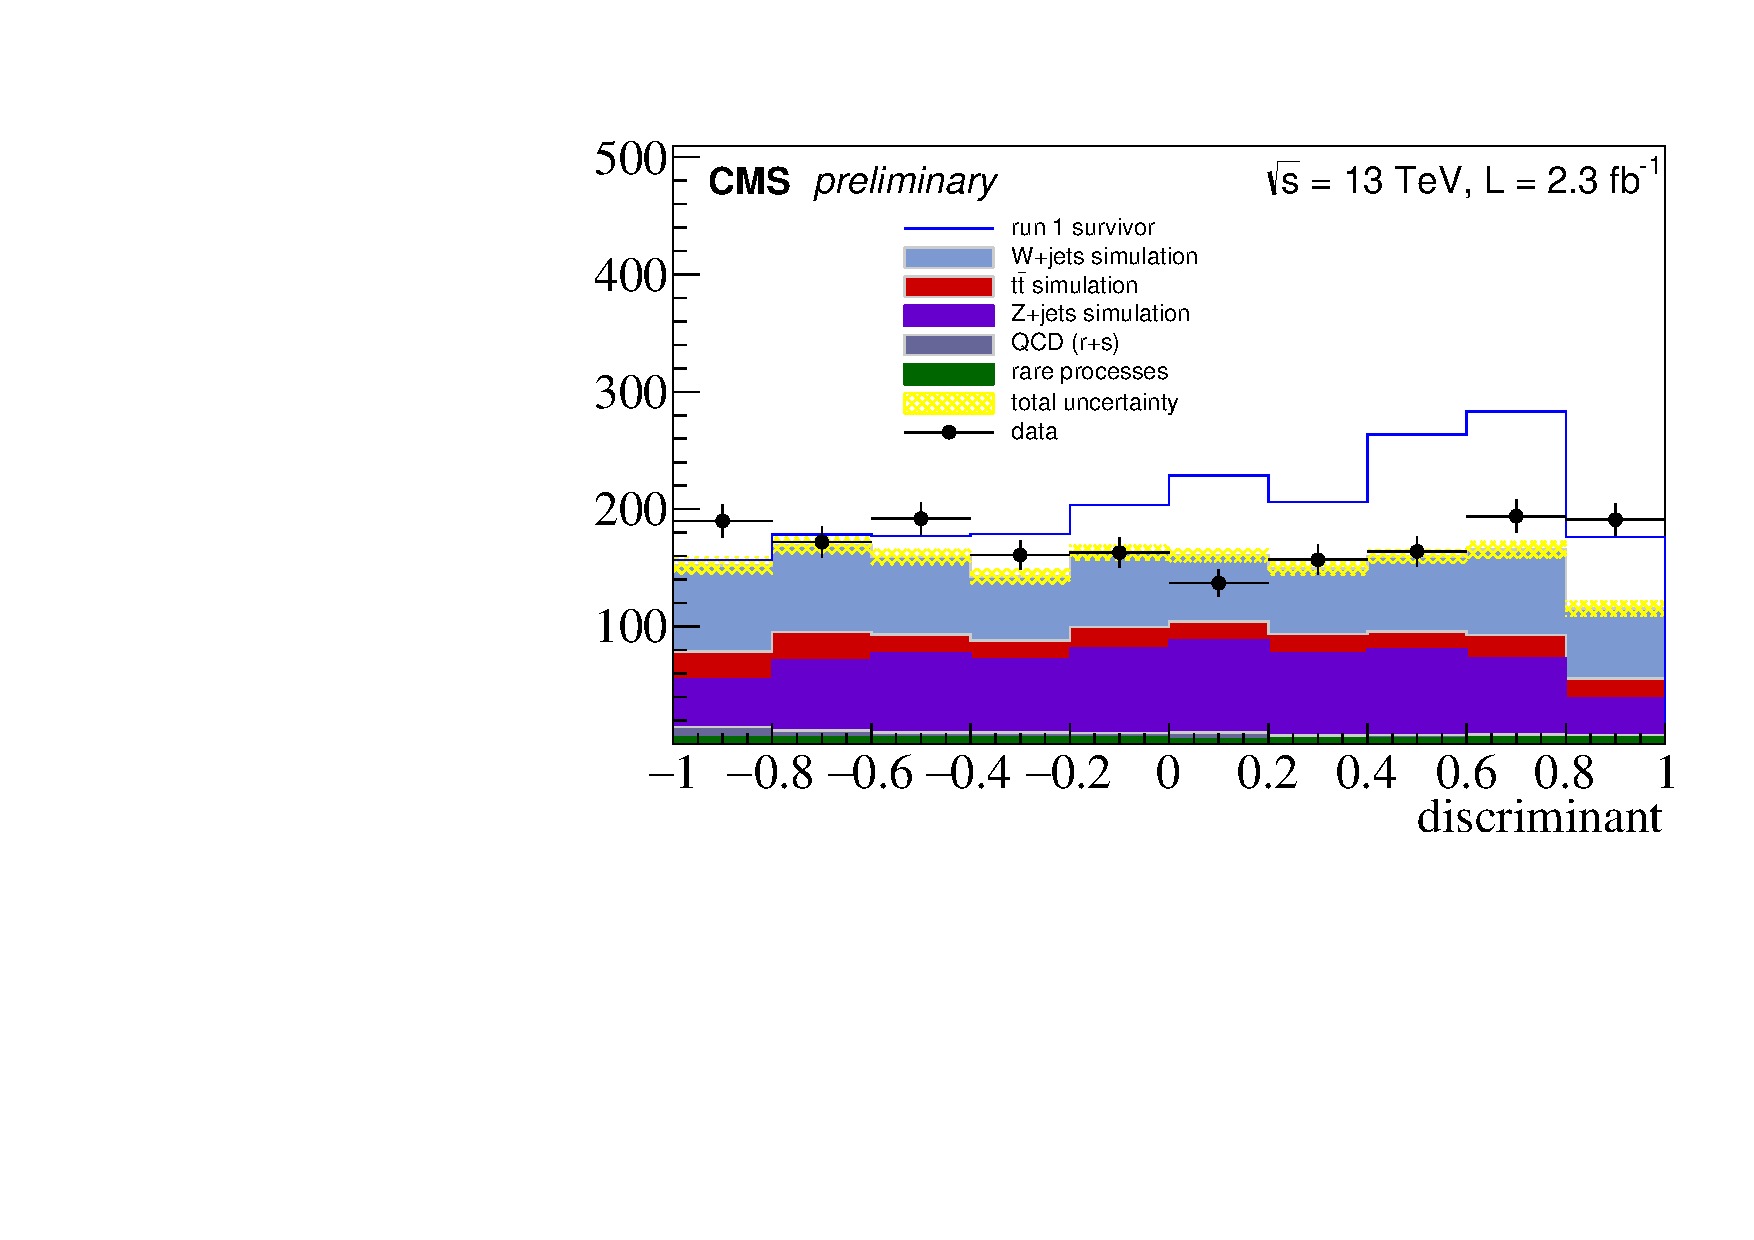
\includegraphics[width=0.65\linewidth]{figures/SusySearches/MvaSusy/ResultMC.pdf}
\caption{Predicted and observed counts for the low-$\Ht$ search using the fully data-driven prediction (top), as well as the prediction from pure simulation (bottom), shown for comparison. The yellow bands are the total uncertainties in the data-driven prediction (top), and the purely statistical uncertainties in the simulated counts (bottom).}
\label{fig:results}
\end{figure}
The results are interpreted using a ``counts'' likelihood, similar to that described in Section \ref{sec:cmslhd}, given by  
\begin{equation}
L(D^\mCMS|\theta\,) = \prod_{i=1}^9 \int \textrm{Poisson}(N_i | s_i+ b_i) \, p(b_i|B_i, \delta B_i) \, p(s_i|S_i, \delta S_i) db_i\, ds_i,
\label{eq:lhd_counts}
\end{equation}
where the product is over the 9 signal regions. For each search bin $i$, $N_i$ is the observed count,
$s_i$ and $b_i$ are the expected number of signal and background counts, respectively,
 $B_i \pm\delta B_i$ is the estimate of the background count and its uncertainty, and 
 $S_i \pm\delta S_i$ is the estimate of the signal count and its uncertainty.
The prior density for $b_i$, $p(b_i|B_i, \delta B_i)$, is modeled as a gamma density, 
$\textrm{gamma}(x;\alpha,\beta) = \beta \exp(-\beta x)  (\beta x)^{\alpha-1}/\Gamma(\alpha)$,
with $\alpha$ and $\beta$ defined such that the mode and variance of the gamma density are 
$B_i$ and $(\delta B_i)^2$. An analogous prescription is used for the signal prior. 
The signed significance $Z$ described in Section \ref{sec:cmslhd} is also computed, where $Z<-1.64$ indicates exclusion at the
95\% CL, and $Z>>0$ indicates evidence for the signal hypothesis with a significance equal to $Z$.

The expected value of $Z$ under the background-only hypothesis is $-5.16$, indicating an expected exclusion of the benchmark model with a significance of approximately 5 standard deviations. The expected $Z$ under the background $+$ signal hypothesis is $4.69$, indicating that, if the signal hypothesis were true, I would expect to observe evidence for the signal with a significance of approximately 4 standard deviations. The observed $Z$-significance is $-3.58$, indicating that the benchmark model is excluded at a significance of about 3 standard deviations. The observed exclusion is weaker than the expected exclusion because of observed excesses over the predicted counts in the most sensitive signal regions.

The benchmark pMSSM point, which survived previous CMS analyses, has been excluded. This preliminary analysis stands as a demonstration that, given a willingness to adopt new techniques, we can look for supersymmetry in the most background-dominated kinematic regions, where evidence of new physics may be manifest. If supersymmetry is not discovered at high-$\Ht$ and high $\mht$, these regions and techniques may be key to ruling out, or providing evidence for, weak-scale supersymmetry at the LHC.


\subsubsection{A note on the discrimination power}
It is possible that providing more sophisticated variables as input to a multivariate discriminant could result in better performance than that achieved by the discriminants discussed here. Appendix \ref{app:discriminators} gives a brief introduction to a few such observables, some of which have been central to CMS and/or ATLAS searches for supersymmetry. Studies that evaluate the effectiveness with which these observables probe the pMSSM, taken alone and in combinations with each other, may prove informative. Also, training with a larger sample of background events may increase the separation power of the discriminant. 




